\documentclass[10pt,twoside,lineno]{gsajnl}
\articletype{inv} % article type

\usepackage{xcolor}
\usepackage{amsmath}
\usepackage{amssymb}
\usepackage{natbib}
\usepackage[linesnumbered,ruled,vlined,algo2e]{algorithm2e}
\usepackage{tikz}
\usetikzlibrary{arrows, snakes,backgrounds}
\tikzstyle{place}=[circle,draw=black,thick, inner sep=0pt, minimum size = 5mm]

\SetKwInput{input}{Input}
\SetKwInput{output}{Output}

\newcommand{\E}{\mathbb{E}}
\renewcommand{\P}{\mathbb{P}}
\newcommand{\R}{\mathbb{R}}
\newcommand{\tn}{\textnormal}
\newcommand{\ov}{\overline}
\newcommand{\tskit}{\texttt{tskit}}
\newcommand{\comment}[1]{{\color{blue} \it #1}}


\title{
    Information in recombination junctions 
    can both compress and improve inferred tree sequences
}

% Non-coalescing regions of dark matter in ARGs
% Can we find them? Are they useful in inference, dating? 
% Look, we can find them and they seem at least useful for compression.
% Also, here's a way of measuring agreement that takes this sort of thing into account,
%  which extends R-F to measure haplotypes


% NOTE: these are in alphabetical order for now; we can revisit that ordering
\author[$\dagger$]{Ava Bamforth}
\author[$\dagger$]{Halley Fritze}
\author[$\ddagger$]{Jerome Kelleher}
\author[$\dagger$]{Nathaniel Pope}
\author[$\ast$,$\dagger$,1]{Peter Ralph}

\affil[$\ast$]{Institute of Evolution and Ecology and Department of Biology, University of Oregon, Eugene, Oregon}
\affil[$\dagger$]{Department of Mathematics, University of Oregon, Eugene, Oregon}
\affil[$\ddagger$]{Big Data Institute, Li Ka Shing Centre for Health Information and Discovery, University of Oxford}


\keywords{genealogy, tree sequence, haplotypes}

\runningtitle{Junctions in tree sequences}
\runningauthor{Bamforth \textit{et al.}}

%%%%%%%%%%
\begin{abstract}
    Foreshadowing haplotype-based methods of the genomics era,
    it is an old observation that the ``junction'' between two distinct haplotypes
    produced by recombination is inherited as a Mendelian marker.
    In this paper, we describe how this recombination-mediated information
    can in many cases be recovered from inference based solely on
    polymorphic markers (i.e., information produced by mutation),
    which produces unary nodes along the branches of the marginal genealogical trees.
    The resulting inferred ARGs, represented as tree sequences,
    are smaller, faster to compute with,
    and potentially contain substantially more information
    about the age of ancestral haplotypes,
    than inferred ARGs without these unary nodes.
    We provide efficient algorithms to identify this ancestral haplotype information,
    new metrics of agreement/disagreement between inferred ARGs,
    and explore some consequences for ARGs inferred from real data.
\end{abstract}

\begin{document}

\maketitle
\thispagestyle{firststyle}
\marginmark
\firstpagefootnote

\correspondingauthoraffiliation{1}{Corresponding author: {plr@uoregon.edu}}
\vspace{-33pt}% Only used for adjusting extra space in the left column of the first page

\comment{idea: look at ratio of unary-to-not over time; does it change with
    selection? or modes of recombination?}

%%% OUTLINE
% Intro: haplotypes, unary bits of non-coalescing nodes, ARGS, etcetera
%    explain what tsinfer does to create unary regions
%    statement of problem
%    Yan: are breakpoints in true->simplify->extend the same as in original?
%   Fig 1: conceptual figure
%    Also IBD gets screwed up
% 
% Methods:
%   edge extend algorithm
%   discrepancy funciton algorithm
%   Fig 2: Conceptual figure for discrepancy
% 
% Results:
%   Fig 3:
%     (a) reduction in number of edges and (b) speed change
%
%   Fig 4:
%     Histograms of (a) total span added, (b) percent incorrect
%
%   Fig 5 and maybe 6: how it interacts with tsinfer
%     (a) summarize total matching and unmatching span (or maybe percent matching?)
%           across reps
%     (b) discrepancy per node against depth or time or number of subtended samples
%        describe percent span matched against true span or depth or something
%
%   Fig 7(?): compare IBD stats before/after
% 
% Supp:
%   S1: runtime
%%%


% Name ideas:
% 
% extend edges
% bundle edges
% inflate edges
% bundle lines of descent
% longer ancestral haplotypes
% inflated ancestors
% compress paths
% optimizing edge tables
% reduce number of ancestors
% reduce ancestral paths

\section{Introduction}

% PETER
% * what's a tree sequence
% * why is a tree sequence (motivation)

There has been substantial recent progress
in the problem of ``ARG inference'',
which seeks to infer (portions of) the ``ancestral recombination graph'' (or, ARG)
that describes how a set of genotypes samples are related to each other
at each position of the genome.
For reviews of this progress, see CITE CITE CITE.
Often such methods focus on the sequence of ``marginal trees'',
i.e., the genealogical trees that describe how each portion of the genome
was inherited by the focal genomes.
For instance, the ``succinct tree sequence'',
introduced by \citet{kelleher2016efficient},
is a common format for describing these inferred ARGs,
and is seeing wide use thanks in part to its efficiency and accompanying reliable toolkit,
\tskit (CITE).

However, the ARG is emphatically not merely a sequence of trees:
since each segment of an ancestor's genome that has been inherited by the focal genomes
may extend over a portion of the genome over which there are many distinct trees,
a single ancestor should usually be represented by nodes in many distinct trees.
In other words, one way to view an ARG is as a sequence of trees in which nodes may be shared across many trees,
but another way to view the ARG is as a set of relationships between segments of ancestral haplotypes.

Another reason we tend to focus on the trees is that
much of our intuition about inference of relationships from genomic data
comes from phylogenetics.
Indeed, all methods might very roughly be summarized as
``more similar sequences are more closely related''.
For instance, two sequences that share a drerived mutation
are (probably) more closely related over some span of genome surrounding the location where the mutation occurs.
\citet{fisher} pointed out that not only mutations
but also the ``junctions'' between distinct haplotypes,
if they could be somehow identified,
would be inherited as Mendelian markers.

\subsection{Motivation and statement of problem}

% PETER
% * minimize number of edges
% * gives extra info about shared haplotypes, reduces number of ancestral paths

Consider the (small portion) of a hypothetical tree sequence in Figure~\ref{fig:conceptual}A.
On the first portion of the genome (left-hand tree), the sample nodes (labeled 0, 1, and 2)
coalesce into a small subtree: 1 and 2 find a common ancestor in ancestral node 3,
which finds a common ancestor with node 0 in ancestral node 4.
On the next portion of the genome (right-hand tree), sample node 2 has a different ancestor.
This seems reasonable, and a method that infers trees separately on each portion of the genome
could not be expected to produce anything different.
However, things change once we think about what this implies about haplotype inheritance.
Figure~\ref{fig:conceptual}B shows the implied inheritance of haplotypes,
with the haplotypes carried by 4 to the left and right of the recombination breakpoint labeled $L$ and $R$.
Here, sample node 2 has inherited the chunk of haplotype labeled $L$ from ancestral node 4 via 3,
and the haplotype to the right of this from some other node (and so doesn't carry haplotype $R$).
On the other hand, sample node 1 has inherited \emph{both} haplotypes $L$ and $R$
from ancestral node 4, but the trees imply that only haplotype $L$ is inherited via ancestral node 3.
This implies -- if taken literally -- that there must have been a recombination event
at some point between node 1 and node 4 that separated the $L$ and $R$ haplotypes,
and then these two ancestral (and nonoverlapping) haplotypes coalesced together in ancestral node 4.
Although this is possible, it seems unlikely --
a more parsimonious explanation is depicted in Figure~\ref{fig:conceptual}C,
in which sample node 1 inherits the entire $LR$ haplotype from ancestral node 4 through node 3
(and there is a recombination somewhere between node 3 and node 2).
This implies that ancestral node 3 inherits from node 4 on the right-hand tree as well,
which is depicted in Figure~\ref{fig:conceptual}D --
and so node 3 has become unary in this tree.
Note that the more parsimonious tree sequence also includes fewer edges:
the three distinct edges $4 \to 3$, $3 \to 1$, and $4 \to 1$ in Figure~\ref{fig:conceptual}B
have been reduced to the two edges
$4 \to 3$ and $3 \to 1$ in Figure~\ref{fig:conceptual}D.

\begin{figure}
    \begin{center}
    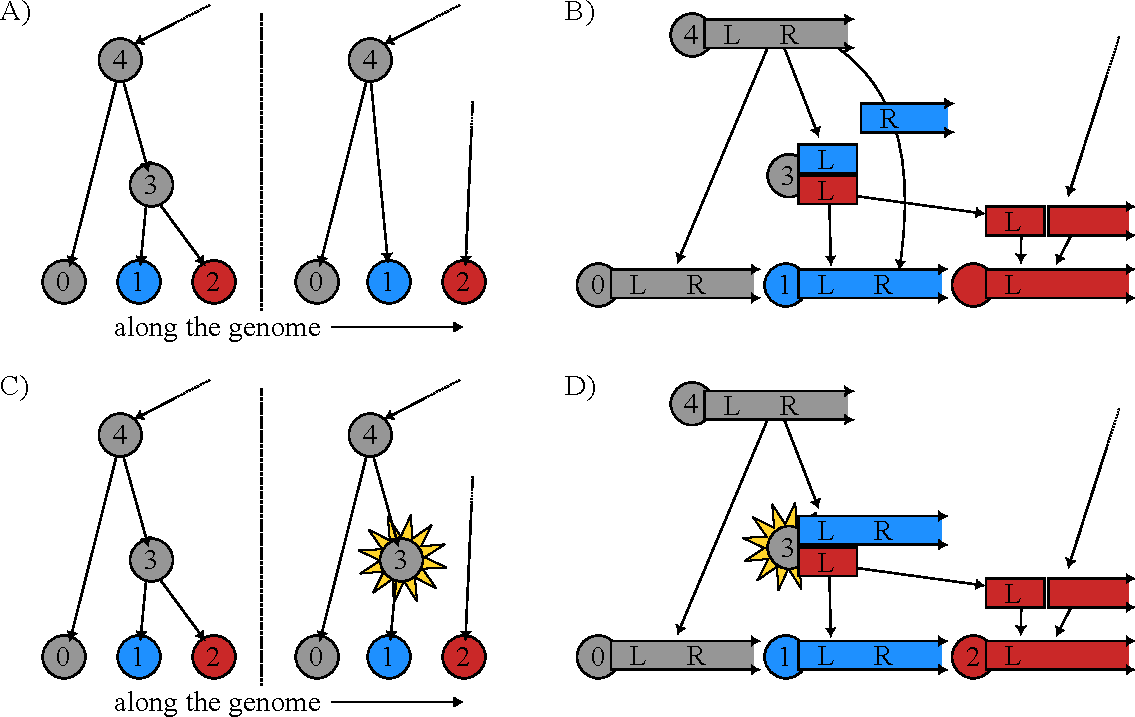
\includegraphics[width=0.9\textwidth]{conceptual_figure}
    \end{center}
    \caption{
        A simple example showing the basic idea
        (described in more detail in the text):
        \textbf{(A)} a small portion of a tree sequence without unary nodes;
        \textbf{(B)} the implied inheritance pattern of the two portions of the haplotype carried by ancestral node 4,
        labeled $L$ and $R$;
        \textbf{(C)} marginal trees with a unary node added,
        which produces \textbf{(D)} a more parsimonious haplotype inheritance pattern
        (that also includes fewer edges).
        \label{fig:conceptual}
    }
\end{figure}

\section{Methods}

\subsection{Algorithm}

% * description (HALLEY)
% * proof of something:
%     - arrives at a local minimum?
%     - guess at typical reduction? (reduces edges by 1/3?)
 
\subsection*{Notation}
    We begin with some notation. We define a \textit{tree sequence}, denoted $TS$, 
    as a tuple $\left( \left\{T_k\right\}, N, E, L\right)$ where
     $\left\{T_k\right\}_{k=1}^n$ is the set of trees,
     $N$ and $E$ are the sets of nodes and edges respectively,
     and $L=[0,a)\subseteq \R$ is the length of the sequence on the genome.
     The length of each tree $T_k$ is some subinterval $[a_k,a_{k+1})$ 
     with the lengths of consecutive trees in the sequence 
     only intersecting each intervals endpoints. 
    Additionally, a node $x\in N$ is \textit{unary} if it only has one child, 
    ie. only a single edge extending below it on the tree.
    With these tree sequences our goal is to
    minimize the number of edges
    as well as infer coalescence of genes. 
    To remove edges we consider the following example.
    Suppose for a tree $T_k$ in the tree sequence $TS$ 
    there exists a branch which contains a unary node $b\in N$.
    Then the node $b$ has one parent, $a\in N$, 
    and one child $c\in N$,
    each with edges $e_{ab}, e_{bc}\in E$ connecting them.
    If there is an edge between the nodes $a$ and $c$ in trees 
    $T_{k+1}$ (or $T_{k-1}$),
    then we wish to extend the edges $e_{ab},e_{bc}$ 
    to $T_{k+1}$ and then remove the edge $e_{ac}$ from $T_{k+1}$. 
    This action reduces the length of the edge $e_{ac}$ on the genome,
    and in some cases, completely removes the edge. 
    We now perform this action on all such unary nodes 
    over the entire tree sequence.

\begin{figure}
\begin{center}
\begin{tikzpicture} 
	\node[circle,draw,inner sep=1pt] (a) at (0,2) {a}
	[growth parent anchor=south] 
		child { node[circle,draw,inner sep=1pt] {b} 		
	 			child {
	 				node[circle,draw,inner sep=1pt] (c) at (0,0) {c}
	 					child{node (d) at (0,1) {$T_k$}
	 						edge from parent [draw=none]}
	 				edge from parent 
	 					node[left] {$e_{b,c}$}
	 			}	 		
	 		edge from parent
	 			node[left] {$e_{a,b}$}
	 	};
 	
	 	
	\node[circle,draw,inner sep=1pt] (a') at (3,2) {a}
	[growth parent anchor=south]
		child {
			child{
				node[circle,draw,inner sep=1pt] (c') at (0,-0.25) {c}	
					child{node (d) at (0,1) {$T_{k+1}$}
						edge from parent [draw=none]}
			}
			node[left] {$e_{a,c}$}
		};	
	
	\node at (6,0) {$\Longrightarrow$};
	\node at (6,0.5) {\tn{Edge Extend}};
	
	\node[circle,draw,inner sep=1pt] (a''') at (9,2) {a}
	[growth parent anchor=south] 
	child { node[circle,draw,inner sep=1pt]	 {b}	
		child {
			node[circle,draw,inner sep=1pt] (c) at (0,0) {c}
			child{node (d) at (0,1) {$T_k$}
				edge from parent [draw=none]}
			edge from parent 
			node[left] {$e_{b,c}$}
		}
		edge from parent
		node[left] {$e_{a,b}$}
	};

	\node[circle,draw,inner sep=1pt] (a'v) at (12,2) {a}
	[growth parent anchor=south] 
	child { node[circle,draw,inner sep=1pt] {b}		
		child {
			node[circle,draw,inner sep=1pt] (c) at (0,0) {c}
			child{node (d) at (0,1) {$T_{k+1}$}
				edge from parent [draw=none]}
			edge from parent 
			node[left] {$e_{b,c}$}
		}
		edge from parent
		node[left] {$e_{a,b}$}
	};
	
	
\end{tikzpicture}
\end{center}
\caption{
    \label{fig:extending_diagram}
}
\end{figure}`


    In more detail, let $TS = \left( \left\{T_k\right\}_{k=1}^n, N, E, L\right)$ 
    be a tree sequence.
    Within tskit we can track a tree sequence using a function called `EdgeDiffs'.
    This function tracks edges which are removed and added 
    between consecutive trees in the sequence. 
    As in \ref{} (tikzfigure), we can track if 
    $e_{a,b}$ and$e_{b,c}$ were removed from $T_k$ 
    when creating $T_{k+1}$, 
    and we can see if $e_{a,c}$ was just added in $T_{k+1}$.


\begin{algorithm2e}[!ht]  % How 'code-like' do we want the algorithm to be? Do we want to keep a lot of the syntax in layman's terms or do we want to use functions like ts1.coiterate(ts2)??
	
\SetStartEndCondition{ }{}{}%
\SetKwProg{Fn}{def}{\string:}{}
\SetKwFunction{Range}{range}%%
\SetKw{KwTo}{in}
\SetKwFor{For}{for}{\string:}{}%
\SetKwIF{If}{ElseIf}{Else}{if}{:}{elif}{else:}{}%
\SetKwFor{While}{while}{:}{fintq}%
\SetKw{Break}{break}
\newcommand\forcond{$i$ \KwTo\Range{$n$}}
\AlgoDontDisplayBlockMarkers\SetAlgoNoEnd\SetAlgoNoLine%

\caption{Extends edges across a tree sequence $TS$.}\label{alg:edge}
\SetKwFunction{ex}{Extend Edges}
\SetKwFunction{fwd}{Forward Extend}
\DontPrintSemicolon
\LinesNotNumbered
%\SetAlgoNoEnd
\input{A tree sequence $TS$}
\output{New tree sequence,$TS'$, with reduced number of edges}

\BlankLine 

\Fn{\fwd (tree sequence $TS$, forwards = \tn{True})}{
{	
\eIf{forwards=\tn{True}}{EdgeDiffs $\gets TS$.edgediffs()\BlankLine}
{\BlankLine
	EdgeDiffs $\gets$ reversed($TS$.edgediffs())\;}
}
\Indm \For{(Interval, EdgesOut, EdgesIn) \KwTo EdgeDiffs}{
	\For{e1 \KwTo EdgesOut}{
		\For{e2 \KwTo EdgesOut}{
			\If{e2.parent = e1.child}{
				\For{e3 \KwTo EdgesIn}{
					\If{e3.parent=e1.parent \tn{AND} e3.child=e2.child}{
						e1.right $\gets$ Interval.right\;
						e2.right $\gets$ Interval.right\;
						e3.left $\gets$ Interval.right\;
						\If{e3.left = e3.right}{
							$E$.remove(e3)\;
							}}}}}}}\;
$TS'\gets TS$.update()\;						
\KwRet{$TS'$}\;
}
\BlankLine						
\Fn{\ex ($TS$, iter=100)}{
	edges $\gets$ $TS$.numedges()\;
	\BlankLine
	\For{$*$ \KwTo \Range(iter)}{
		$TS' \gets TS$.\fwd(fowards=\tn{True})\;
		$TS' \gets TS$.\fwd(fowards=\tn{False})\;
		\eIf{$TS$.numedges = edges}{
			\Break\BlankLine}
		{edges $\gets$ $TS'$.numedges()\;}
		}
}
\KwRet{$TS'$}\;
\end{algorithm2e}

With this algorithm we only extend existing edges
over a larger interval on the genome,
and remove unnecessary edges in the process.
%% Find counter example to global minimum.

\subsection{Discrepancy Function}
% * How to measure agreement that includes haplotypes
% * Definition and Algorithm
% * Supp fig: runtime ~ # trees, samples
% * fig: how add edges reduces discrepancy (RESULTS)
%       - compare to tsinfer
% * Show: how add edges reduces discrepancy (RESULTS)
% * THINK of a way to asynchronously computing discrepancy (???)

\par Now with an algorithm in place
 we need a metric to discern
 if trees modified with edge extend
 in fact correctly infer haplotypes in our original tree sequence.
 We have thus constructed a function which counts the differences 
 between trees on a pair of tree sequences. 
 To count all the discrepancies we must begin by counting differences for each node in the tree sequence.

\begin{figure}
    \caption{
        Conceptual figure displaying what discrepancy is?
        TODO: brainstorm.
        \label{fig:conceptual_discrepancy}
    }
\end{figure}

 Let $TS^1=(\{T_i^1\},N^1,E^1,L^1)$ and $TS^2=(\{T^2_j\},N^2,E^2,L^2)$ be tree sequences.
 Suppose that $x\in N^1$ and $y\in N^2$ are nodes in each tree sequence.
 We denote the \textit{set of descendant samples} of $x$ at position $i$ in the genome as $D_{TS^1}(x,i)$.
 Now for a pair of nodes $(x,y)\in TS^1\times TS^2$ 
 we can measure how much they agree along the genome.
 We do so with the following function
 $$\rho_{(TS^1,TS^2)}(x,y)=\frac{1}{L}\sum_{i=0}^{L-1}[D_{TS^1}(x,i)=D_{TS^2}(y,i)],$$
 where $L=\min\{L^1,L^2\}$ and $[\cdot]$ is the characteristic function. 
 We see $\rho$ measures the fraction of the tree sequence
 along which $x$ and $y$ have exactly the same descendant set. 
 For each node $x\in N^1$ we can use $\rho$ to find its global best matching node $y\in N^2$. 
 This node $y$ should not just be a maximum of $\rho(x,\cdot)$ but it should also have a branch length similar to $x$. 
 This means our node $y$ should minimize both $|t_x-t_y|$ and $1-\rho_{(TS^1,TS^2)}$.
 We then use this $y$ to find count the length of genome which $x$ differs from its best matching node in $TS_2$ with the function
 $$\hat{d}(x,TS^1,TS^2)=\min_y\{|t_x-t_y|(1-\rho_{(TS^1,TS^2)}(x,y))\}.$$
 Here $t_x$ and $t_y$ denote the time of occurrences (ie. branch length) for nodes $x$ and $y$. 
 The function $\hat{d}$ measures the proportion of the genome 
 over which the descendant set of $x$ differs from its best matching node $y$.
 We can now extend this from any node $x\in N^11$ to all of $TS_1$ with the \textbf{discrepancy function}
 $$d(TS_1,TS_2)=\sum_{x\in N_1}\hat{d}(x,TS_1,TS_2).$$
 This function, as we will see in the algorithm below,
 is $|N^1||\{T^1\}|$ as for each tree in $TS_1$ and each node $x\in N^1$ we only need to look at $O(1)$ nodes rather than all nodes in $N^2$.
 


% PLR: commented this out since it's not compiling
% 
% \begin{algorithm}[!ht]
% \SetStartEndCondition{ }{}{}%
% \SetKwProg{Fn}{def}{\string:}{}
% \SetKwFunction{Range}{range}%%
% \SetKw{KwTo}{in}
% \SetKwFor{For}{for}{\string:}{}%
% \SetKwIF{If}{ElseIf}{Else}{if}{:}{elif}{else:}{}%
% \SetKwFor{While}{while}{:}{fintq}%
% \SetKw{Break}{break}
% \newcommand\forcond{$i$ \KwTo\Range{$n$}}
% \SetKwComment{Comment}{}{} 
% \DontPrintSemicolon
% \LinesNotNumbered
% \AlgoDontDisplayBlockMarkers\SetAlgoNoEnd\SetAlgoNoLine%
% 
% 
% \input{$(TS_1,TS_2)$}
% \output{discrepancy number (some float value)}
% 
% \Fn{Node Discrepancy($x,TS_1,TS_2$)}{
% $s=0\in \mathbb{Z}^{|N^2|}$ \Comment*[f]{Similarity vector with each entry corresponds to a node in $TS_2$}
% 
% \For{$I$, $T^1_k$, $T^2_j$ \KwTo $(L,TS_1,TS_2)$}{
% \Comment{Here $I=[a^1_k,a^1_{k+1})\cap [a^2_j,a^2_{j+1})$ is the interval which the two trees $T^1_k$, $T^2_j$ both span over. Here we find the best matching node $y$.}
% $D_{T^1_k}(x)\gets D_{TS^1}(x,i)$ where $i\in I$\;
% \If{$|D_{T^1_k}(x)| > 0$}{
% \If{$|D_{T^1_k}(x)|=1$}{
% $y \gets D_{T^1_k}(x)$\;
% $m \gets D_{T^1_k}(x)$\;}
% \Else{$m \gets $ most recent common anscestor of $D_{T^1_k}(x)$ in $T^1_k$\;
% $y\gets $ most recent common anscestor of $D_{T^1_k}(x)$ in $T^2_j$\;}}
% \If{$D_{T^2_j}(y)=D_{T^1_k}(x)$}{
% $s_y\gets s_y$\;}}
% \KwRet{node discrepancy}\;}
% \Fn{Discrepancy($TS_1,TS_2$)}{
% discrepancy = 0\;
% \For{$x\in N^1$}{discrepancy = $\sum_{x\in N^1}{$Node Discrepancy($x,TS_1,TS_2$)}}
% \BlankLine
% \KwRet{discrepancy}}
% \caption{Discrepancy Function}\label{ndisc}
% \end{algorithm}


\section{Results}

\comment{
    Idea: look at statistical properties of unary regions:
    look at how much 'unary regions' there is in simulation
    and how much we can put back in,
    as a function of time.
}

% (AVA)
% * reduction in edges ~ sequence length
% * speed increase ~ sequence length
% * proprotion of added edges that are true ~ sequeence length

\begin{figure}
    \caption{
        Two-part figure, showing reduction in number of edges (left) and increase in speed of stats comptuation (right)
        as a function of number of trees (modulated by sequence length),
        on reasonably big simulated sequences.
        For "speed": plot ratio of runtime before/after extending.
        \label{fig:speed_and_edges}
    }
\end{figure}

Simple experiment:
(1) simulate, simplify, and extend;
(2) let $x$ be total matching span of simplified tree (here equal to the total span); $y$ total matching span of extended tree in truth and $z$ total not-matching span;
then $z$ is "total wrongly added stuff" and $y-x$ is "total rightly added stuff".

With tsinfer: (1) simulate and tsinfer; (2) do the above either with or without simplifying the tsinfer'ed trees.
(but also take into account that there's wrong stuff in tsinfer'ed tree: look at whether it reduces discrepancy!)

\begin{figure}
    \caption{
        Maybe: summaries of lengths and/or numbers of correctly and incorrectly added edges?
        (See notebook.)
        \label{fig:results_edges}
    }
\end{figure}

\subsection{Data}
% * 1. Simulate data
% * 2. Run tsinfer
% * 3. Compare d(x,truth) for x in tsinfer, tsinfer+add edge, tsinfer+add edge + simplify, tsinfer+simplify

% * How much unary edges?
% * How much can we add?

% * apply to real data:
%     - % fewer edges
%     - % fewer distinct ancestors (ancestral paths?) of sample at some time

\section{Discussion}

TODO

\bibliography{references}

\appendix

\begin{figure}
    \caption{
        Supplementary figure: runtime of discrepancy function as a function of number of trees
        (which we modulate by changing sequence length).
        \label{fig:speed_discrepancy}
    }
\end{figure}

\end{document}
